\documentclass[tikz,border=10pt]{standalone}
\usepackage{tikz}
\usetikzlibrary{shapes.geometric}
\usepackage{amsmath}

\begin{document}
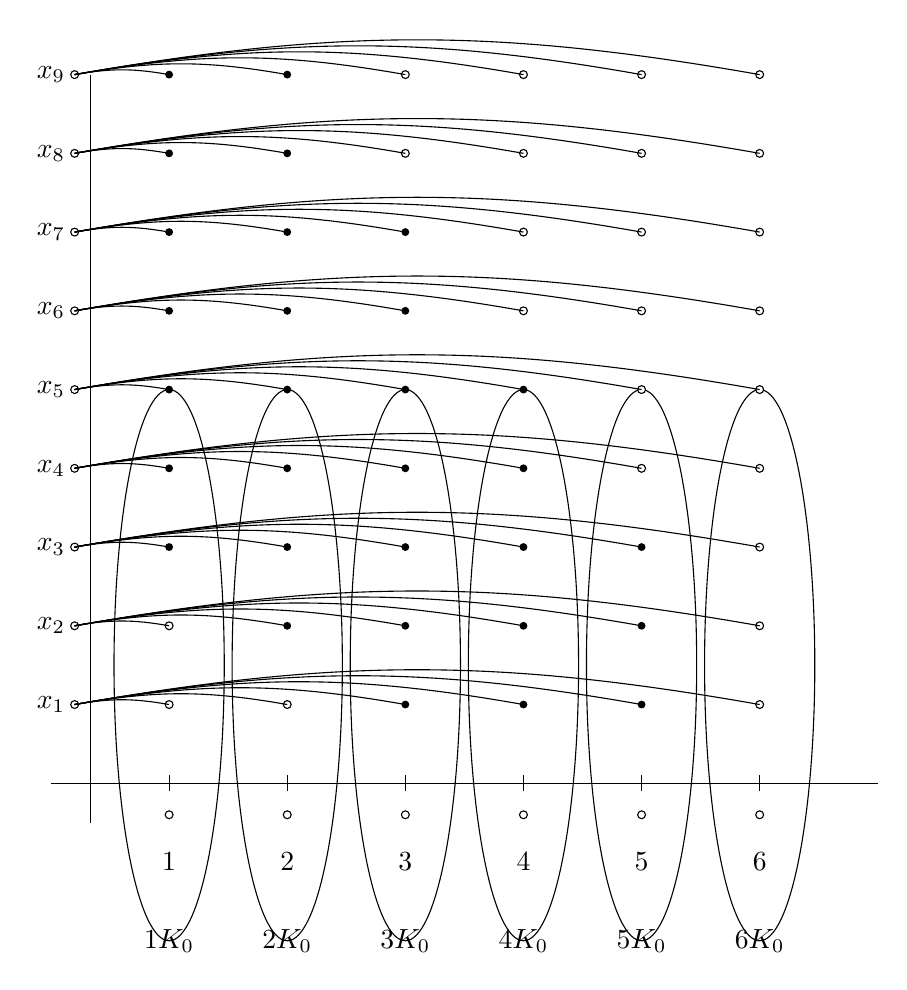
\begin{tikzpicture}[scale=1.0]
  % 定义样式
  \tikzset{
    fillednode/.style={circle, fill, inner sep=0pt, minimum size=0.1cm},
    emptynode/.style={circle, draw, fill=white, inner sep=0pt, minimum size=0.1cm}
  }
  
  % 绘制坐标轴
  \draw (-0.5,0) -- (10,0);
  \draw (0,-0.5) -- (0,9);
  
  % 绘制x轴标签
  \foreach \i in {1,...,6} {
    \node at (\i*1.5-0.5,-1) {$\i$};
    \node at (\i*1.5-0.5,-2) {$\i K_0$};
    \draw (\i*1.5-0.5,-0.1) -- (\i*1.5-0.5,0.1);
    \node[emptynode] at (\i*1.5-0.5,-0.4) {};
  }
  
  % 绘制y轴标签和点
  \foreach \i in {1,...,9} {
    \node at (-0.5,\i) {$x_{\i}$};
    \node[emptynode] at (-0.2,\i) {};
  }
  
  % 绘制椭圆
  \foreach \i in {1,...,6} {
    \draw (\i*1.5-0.5,1.5) ellipse (0.7cm and 3.5cm);
  }
  
  % 第一个椭圆内的点
  \foreach \y in {3,4,5,6,7,8,9} {
    \node[fillednode] at (1,\y) {};
  }
  \foreach \y in {1,2} {
    \node[emptynode] at (1,\y) {};
  }
  
  % 第二个椭圆内的点
  \foreach \y in {2,3,4,5,6,7,8,9} {
    \node[fillednode] at (2.5,\y) {};
  }
  \foreach \y in {1} {
    \node[emptynode] at (2.5,\y) {};
  }
  
  % 第三个椭圆内的点
  \foreach \y in {1,2,3,4,5,6,7} {
    \node[fillednode] at (4,\y) {};
  }
  \foreach \y in {8,9} {
    \node[emptynode] at (4,\y) {};
  }
  
  % 第四个椭圆内的点
  \foreach \y in {1,2,3,4,5} {
    \node[fillednode] at (5.5,\y) {};
  }
  \foreach \y in {6,7,8,9} {
    \node[emptynode] at (5.5,\y) {};
  }
  
  % 第五个椭圆内的点
  \foreach \y in {1,2,3} {
    \node[fillednode] at (7,\y) {};
  }
  \foreach \y in {4,5,6,7,8,9} {
    \node[emptynode] at (7,\y) {};
  }
  
  % 第六个椭圆内的点
  \foreach \y in {1,...,9} {
    \node[emptynode] at (8.5,\y) {};
  }
  
  % 连接线
  \foreach \y in {1,...,9} {
    \draw[bend left=10] (-0.2,\y) to (1,\y);
    \draw[bend left=10] (-0.2,\y) to (2.5,\y);
    \draw[bend left=10] (-0.2,\y) to (4,\y);
    \draw[bend left=10] (-0.2,\y) to (5.5,\y);
    \draw[bend left=10] (-0.2,\y) to (7,\y);
    \draw[bend left=10] (-0.2,\y) to (8.5,\y);
  }
  
\end{tikzpicture}
\end{document}